\documentclass{article}
\usepackage[utf8]{inputenc}
\usepackage{graphicx} %package to manage images
\usepackage{float}
\graphicspath{ {./Pictures/} }

\title{VizCon User's Guide}
\author{UCF VizCon Team}
\date{March 2022}

\begin{document}

\maketitle

\section{History}
In 2004, Professor Mordechai (Moti) Ben-Ari of the Weizmann Institute of Science released an integrated development environment (IDE) known as jBACI. Its purpose was to simulate concurrency in computing in a manner that could teach students about this concept with ease. This is done through multiple displays that are shown while a program is running in real-time; in particular, concurrency is demonstrated through its processes window. jBACI is quite unique in this aspect, as it is a feature that is not found in other simulators to this day. However, being nearly two decades old, jBACI is largely out-of-date. Problems with it include limited language support (Pascal and C--, neither of which are used today), limited reliability outside of the Windows operating system, and a lack of core features and conventions that are common in modern day IDEs.


VizCon is a reimplementation of jBACI. We have kept all of the features of jBACI that made it useful for educational purposes. However, it is built using modern software and techniques, and it uses an interface and feature set that modern-day programmers will be accustomed to. In addition, it supports macOS and Linux as well as Windows.

\section{Installation and Execution}
On Windows, download and run the .exe file. The program can be uninstalled normally via the Control Panel or Windows app.

On macOS, download and run the .dmg file. On Debian-based Linux distros, download and run the .deb file. On Red Hat-based distros, download and run the .rpm file. 

You must have the following dependencies installed:

$$- gcc >= 8$$

\section{The Integrated Development Environment}
Upon startup, the program will greet you with a Welcome screen shown in Figure 1. 
\begin{figure}[h!]
    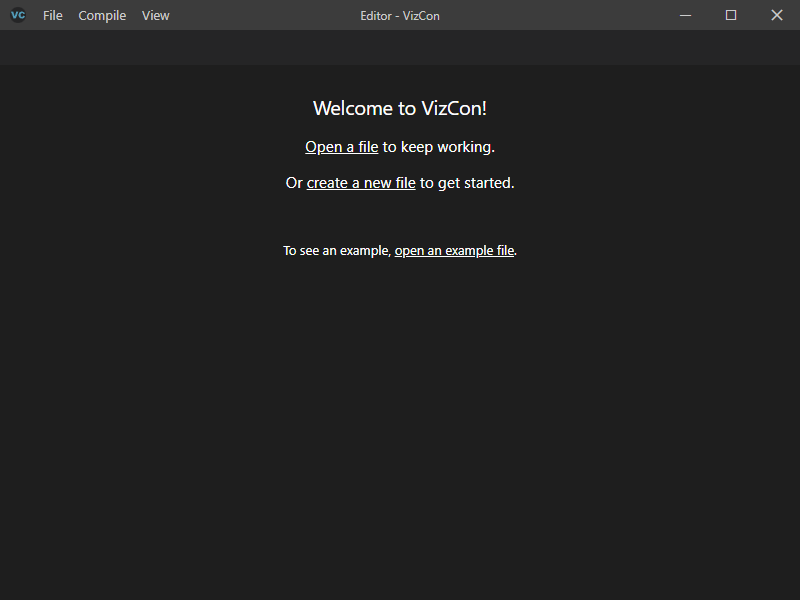
\includegraphics[width=10cm]{vizconWelcomeScreen}
    \centering
    \caption{Welcome screen}
\end{figure}

From the Welcome screen, you have three options: you can create a new file, open an existing file from your last saved opened directory, or open a file from the Examples directory. Every example given is stored in resources/examples.

The toolbar on the top contains the basic menu options expected in an IDE, such as the ability to save or open a file. The keyboard shortcuts for these menu items are listed to the right of the names. The user can also zoom the text in the program in or out. Along with this are additional options exclusive to this program. VizCon's IDE can be separated into two parts: the editor and the visualizer. These components can be toggled between in the View menu.

\subsection{Creating a File}
Upon selecting New File from the menu (ctrl + n) or clicking on 'create a new file' on the welcome screen, an empty file will be made. In order to use VizCon's concurrency functions, the user must include vcuserlibrary.h at the top of the file as shown in Figure 2. 

\begin{figure}[H]
    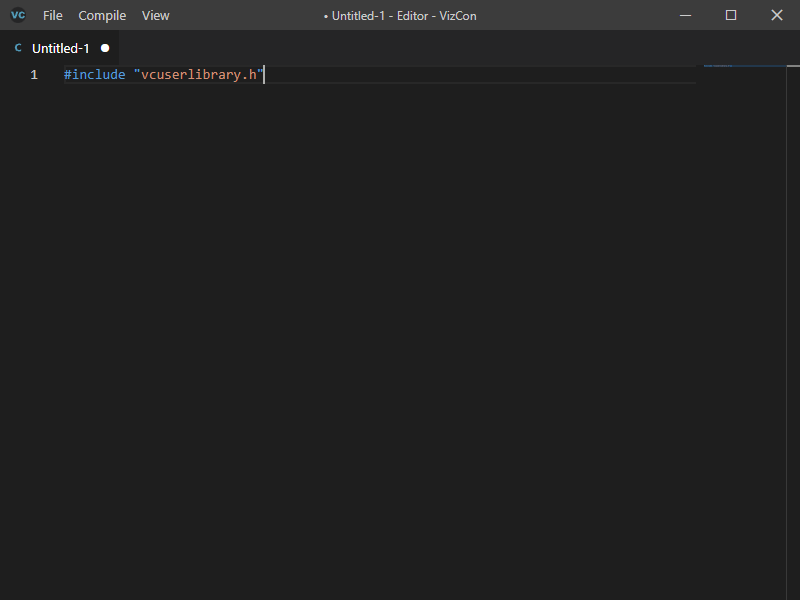
\includegraphics[width=10cm]{vizconHeader}
    \centering
    \caption{A new file with the header library.}
\end{figure}


\subsection{Editing and Compiling}
Figure 3 shows a brief overview of the editor. 
\begin{figure}[h!]
    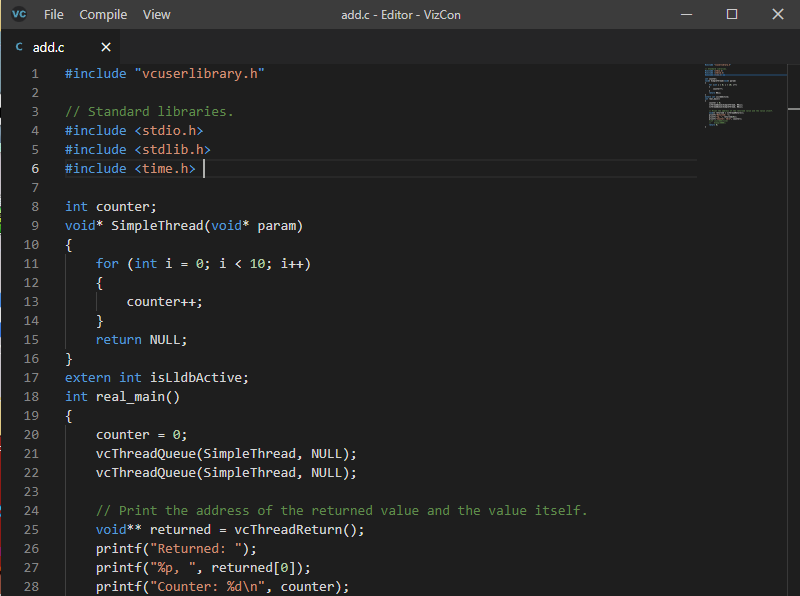
\includegraphics[width=10cm]{vizconEditor}
    \centering
    \caption{VizCon's editor.}
\end{figure}

Shown in the figure is the IDE running one of VizCon's example programs, add.c. The content of the files are shown in a text area, and can be edited as one would expect. Once a program is written, it can either be compiled and run all at once or simply compiled without running from the Compile menu. All source files must be written with the .c extension, as C is the only language that the compiler supports. Compilation output can be shown from the View menu as seen in Figure 4.
\begin{figure}[H]
    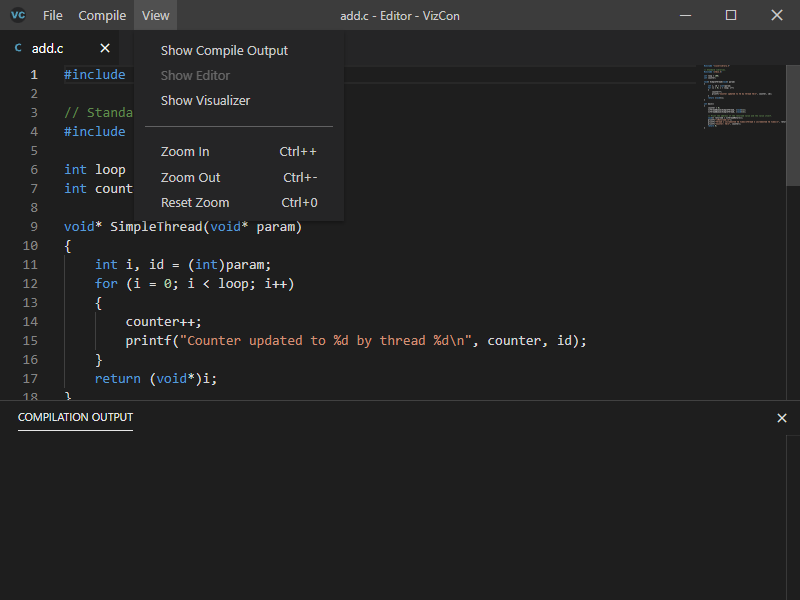
\includegraphics[width=10cm]{vizconCompiler}
    \centering
    \caption{Compilation window.}
\end{figure}

\subsection{Running the Program}
When the Compile and Run option is selected, VizCon switches to its visualizer. Figure 5 shows a brief overview. 
\begin{figure}[H]
    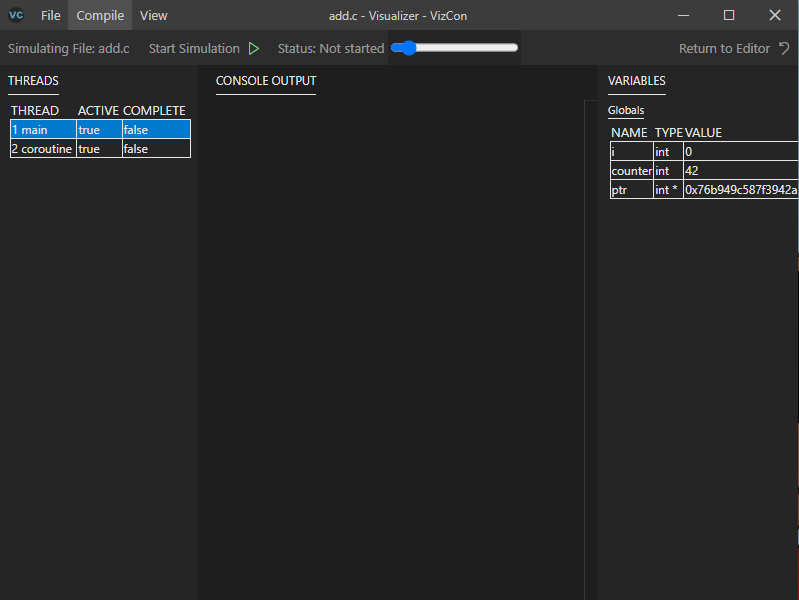
\includegraphics[width=10cm]{vizconVisualizer}
    \centering
    \caption{VizCon's visualizer.}
\end{figure}

The threads in the program are shown in the left column, along with whether or not that thread is currently active and if it has completed. The compilation output is shown in the middle column. The right column shows all of the variable names in the program, as well as their respective values. In order to run the program, the Start Simulation button must be pressed. The user can return to the editor by pressing the Return to Editor button on the top right, or by showing it in the View menu.

\section{Concurrency Constructs}
\subsection{Data Types}
VizCon's user library (vcuserlibrary.h) provides a set of data types to aid with concurrent programming in a cross-platform manner.
\subsubsection{threadFunc}
A data type representing a function that gets taken in during thread creation.
\subsubsection{VcSem (or VcSemaphore)}
VizCon's built-in semaphore data type. 
\subsubsection{VcMutex}
VizCon's built-in mutex data type.

\subsection{vcThreadQueue}
Prepares a thread instance with the function and arguments.
\subsubsection{Syntax}
\begin{verbatim}
    void vcThreadQueue(threadFunc func, void *arg);   
\end{verbatim}

\subsection{vcThreadStart}
Starts all threads that were created in previous calls to vcThreadQueue.
\subsubsection{Syntax}
\begin{verbatim}
    void vcThreadStart();
\end{verbatim}

\subsection{vcThreadReturn}
Starts all threads that were created in previous calls to vcThreadQueue, and returns their values.
\subsubsection{Syntax}
\begin{verbatim}
    void **vcThreadReturn();
\end{verbatim}

\subsection{vcMutexCreate}
Creates a mutex.
\subsubsection{Syntax}
\begin{verbatim}
    vcMutex vcMutexCreate();
\end{verbatim}

\subsection{vcMutexLock}
Attempt to acquire a lock on the mutex, waiting if it is not yet available.
\subsubsection{Syntax}
\begin{verbatim}
    void vcMutexLock(vcMutex mutex);
\end{verbatim}

\subsection{vcMutexTryLock}
Attempt to acquire a lock on the mutex, returning immediately if it is not yet available.
\subsubsection{Syntax}
\begin{verbatim}
    int vcMutexTrylock(vcMutex mutex);
\end{verbatim}

\subsection{vcMutexUnlock}
Release the lock on a mutex.
\subsubsection{Syntax}
\begin{verbatim}
    void vcMutexUnlock(vcMutex mutex);
\end{verbatim}

\end{document}
